%\begin{figure*}[t!]
\section{Design and Implementation}
\iffalse
This section describes the design and implementation of \ours{} buffer in detail. 
\S~\ref{subsec:overview} overviews the overall architecture of the in-storage buffer under capacitance constraints, and \S~\ref{subsec:lind_sched} presents the I/O scheduling algorithm
to reduce the write traffic in \ours{}.

\subsection{Overview}
\label{subsec:overview}
To satisfy a high demand for storage capacity in modern applications,
the SSDs have become highly scalable with advances in density-increasing techniques. 
The state-of-the-art SSDs provide tens of TBs capacity and this trend is expected 
to continue in the future.
The problem is that the capacitors, an integral component used in SSDs to protect the buffer data
in power outage, is unable to keep up with the significant density increase speed of NAND flash memory. 
The SSD-internal buffer is typically 0.1\% of the storage capacity in size.
To protect the entire buffer of SSD, the capacitors 
should have been improved at the same pace with SSD in density; 
its density has enhanced only at one-fifth speed of SSD density improvement. 
% This density gap between capacitors and memory technologies
% indicates that 
With this density gap, the PLP with full protection is no longer feasible in SSDs; 
it not only severely limits the form factor of SSDs requiring deployment of a large number of capacitors but also significantly increases the manufacturing cost of SSDs. 

\ours{} is designed to efficiently maintain the in-storage buffer under capacitance limitations. 
Table~\ref{tab:ssd_buff_comp} shows the breakdown of the in-storage buffer usage for each component
for 512GB SSD that has an architecture shown in Table~\ref{tab:ssd_config}. 
The user data buffer is employed to fully exploit the underlying flash parallelism.
Hence, it is typically twice the size of all pages that can be programmed in parallel, 
which is 4MB in this setting, while it may vary depending on the design choice. 
The mapping table that translates LPN(logical page number) to PPN(physical page number) 
accounts for 512MB, which corresponds to 97\% of the buffer size. 
Other metadata including mapping table directory uses a total of 10.5MB buffer. 

To overcome capacitance constraints for SSD, \ours{} sacrifices on some durability of mapping table, 
% by only protecting a portion of it, 
while protecting the user data and the metadata other than mapping table with capacitors. 
The user data persistence should be synchronously guaranteed with the host request
to conserve the properties of existing SSDs with PLP. 
For this reason, making a compromise on it can lead to a serious performance penalty in SSD.
On contrary, the requirements for the mapping table update are less stringent;
it does not have to be immediate upon a host request because the address translation is 
necessary only when the associated data is actually programmed to the flash memory. 
This nature allows a room for reasonable trade-off between capacitance and performance,
by effectively maintaining the persisting overhead of mapping table under capacitance constraint. 
Other metadata updates are also asynchronous with the host request, but
they use only a marginal space of the buffer; sophisticating their management mechanism 
for further capacitance saving is cost-ineffective. 

% because the PPN of data is determined when it is flushed to the flash memory. 
% The LPB to PPN translation is required when the data is in flash memory. 
% it can be restored on the reboot. 

% 요청된 데이터를 찾기 위해 사용. 
% 데이터는 보호되고 있는데 인덱스는 잃어버림. 
% ==> 추후 recovery 할 때 반영해주면 됨. 데이터를 쓰면서 업데이트 하거나 '
% ==> 이미 데이터가 플래시에 쓰여져 있다면? 걔는 보호를 해줘야 함. 
% ==> 대신 small write 임. 버퍼링 효과를 늘리면 footprint 를 줄일 수 있음. 

\iffalse
If an SSD has 8 channels and 4 ways per channel with 8KB page size, about 128KB of memory (twicethe  size  of  all  pages  that  can  be  written  in  parallel)  are  usedfor data buffering. This, however, only accounts for 0.02% ofthe volatile DRAM.
maximize the high degree of parallism in SSDs 
during the operation of flash memories 
\fi

% the end of full protection based SSD design 
%The capacitance faces scaling limit 

% mapping table 이 상당히 큰 부분을 차지한다. 
% 사용자 버퍼는 통상 SSD의 병렬성을 활용할 수 있는 정도로만 있으면 된다고 했지만, 
% 최근 다양한 이유로 증가하고 있음. 

\subsection{Least Increase of Dirtiness Scheduling}
\label{subsec:lind_sched}
\fi
\ours{} partially protects a mapping table with limited capacitance.  When the
dirty pages of a mapping table reach more than the maximum number of protected
pages, \ours{} flushes them to flash memory based on the Least-recently Used
(LRU) algorithm.  Because the flush operation does not arise with SSD using
PLP, mitigating the negative impact of  flushing is critical to maintain
performance under capacitance constraints.  To this end, \ours{} uses a
cost-effective scheduling scheme for the in-storage buffer. \ours{}
selectively forces the user data to flash memory, which increases the dirtiness
of the mapping table the least. This scheme reduces a dirty memory footprint of
the mapping table at any given moment by enhancing a locality of
updates.  As a result, the frequency of flush operation for the mapping table
can be greatly reduced. 

\begin{figure}
    \centering{}
    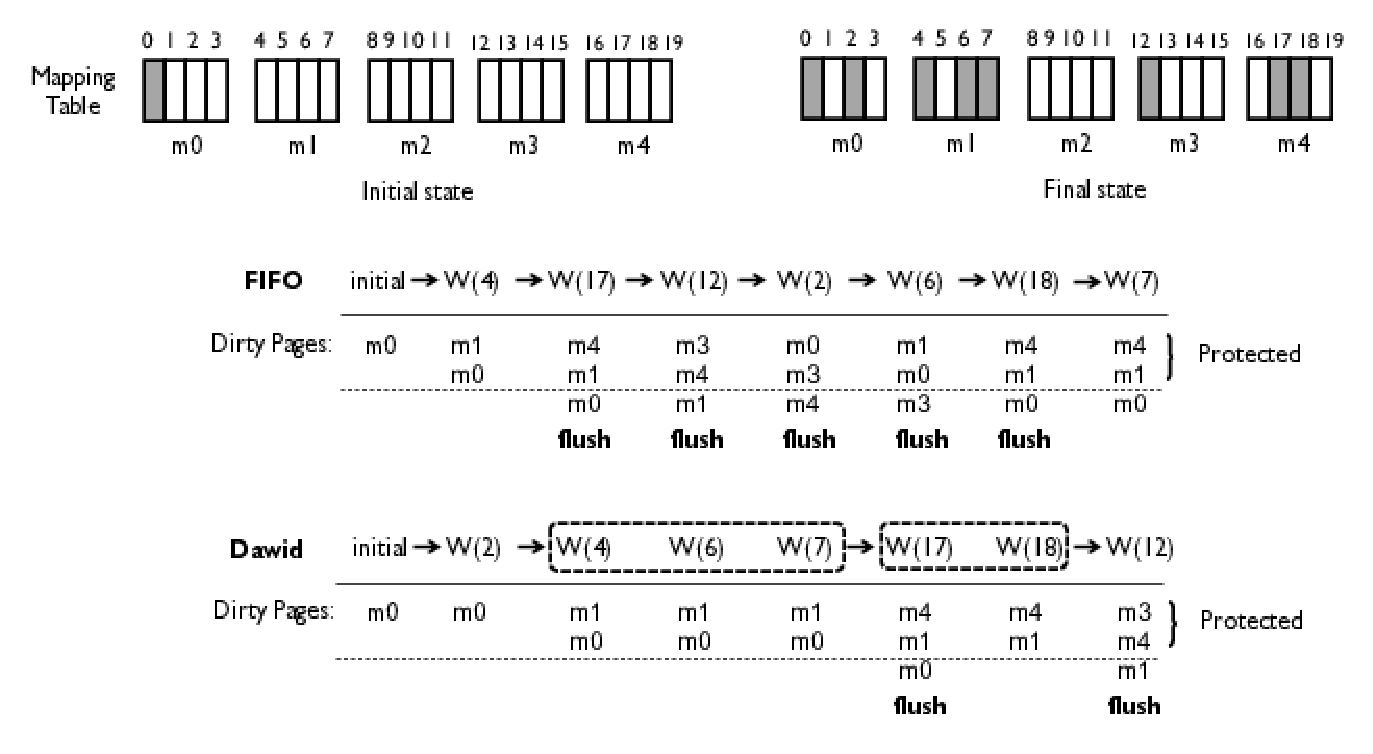
\includegraphics[width=0.5\textwidth]{figure/dawid_algo.eps}
    \caption{\textbf{\ours{} buffer management scheme.}}
    \label{fig:dawid_buff_overview}
    % \vspace{-20pt}
\end{figure}

Fig.~\ref{fig:dawid_buff_overview} compares the flush overhead of FIFO-SSD and \ours{}. 
In this example, there are seven write requests 
in the device queue sent from the host in the following order: \texttt{W(4)}, \texttt{W(17)}, \texttt{W(12)}, \texttt{W(2)}, \texttt{W(6)}, \texttt{W(18)}, and \texttt{W(7)}.  
The mapping table has one dirty page (\texttt{m0}) 
at an initial state. We assume that 2 out of 5 pages of the mapping table are protected. 
FIFO-SSD writes the user data in the buffer to flash memory in arrival order. 
With this scheme, the mapping table would be randomly updated, generating a large number of dirty pages at a 
time window. 
Consequently, FIFO-SSD incurs a total of five flushes of the mapping table page during the write process. 


In contrast, \ours{} calculates the write cost for each datum that indicates an
increase in the number of dirty pages of the mapping table when it is flushed,
and it processes the request with minimum cost first.  In this example, the
write request \texttt{W(2)} has top priority because its associated mapping
table page (\texttt{m0}) is already dirty, and thus it does not add to the number of dirty
translation pages.  Next, the write requests \texttt{W(4)},
\texttt{W(6)}, and \texttt{W(7)} are processed.  Because their address mapping
entries are on the same page of the mapping table, the cost of flushing
them is reduced to one third.  With this scheme, \ours{}
%can reduce the footprint of mapping table updates within time intervals, thereby delivering 
delivers only two flushes of the mapping table for the same task. 

\iffalse
\subsection{Eviction Policy}
\begin{figure}[t!]
    \centering{}
	\subfloat[JESD] { 
    	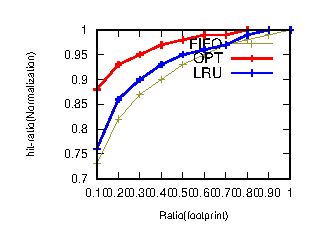
\includegraphics[width=0.2\textwidth]{expr/hitMap/eps/JESD_FIFO.eps}
    	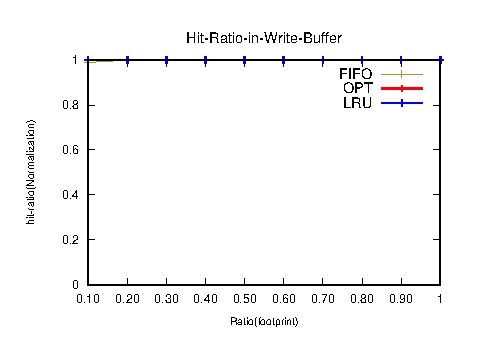
\includegraphics[width=0.2\textwidth]{expr/hitMap/eps/JESD_DAWID.eps}
	} \\
	\subfloat[OLTP]{ 
    	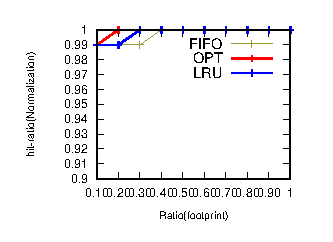
\includegraphics[width=0.2\textwidth]{expr/hitMap/eps/OLTP_FIFO.eps}
    	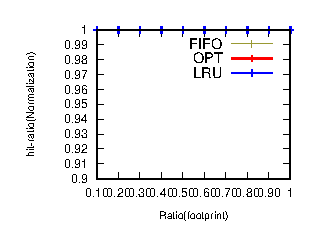
\includegraphics[width=0.2\textwidth]{expr/hitMap/eps/OLTP_DAWID.eps}
	} \\
	\subfloat[Linkbench]{ 
    	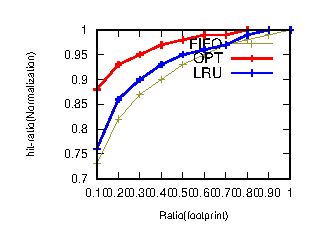
\includegraphics[width=0.2\textwidth]{expr/hitMap/eps/JESD_FIFO.eps}
    	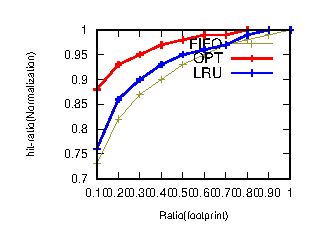
\includegraphics[width=0.2\textwidth]{expr/hitMap/eps/JESD_FIFO.eps}
	} \\
    \caption{\textbf{Write hit ratio for the protected range in a mapping table.}}
    \label{fig_dawid_archi}
\end{figure}
\fi

\begin{figure}[t!]
    \centering{}
% 	\subfloat[Architecture] { 
%     	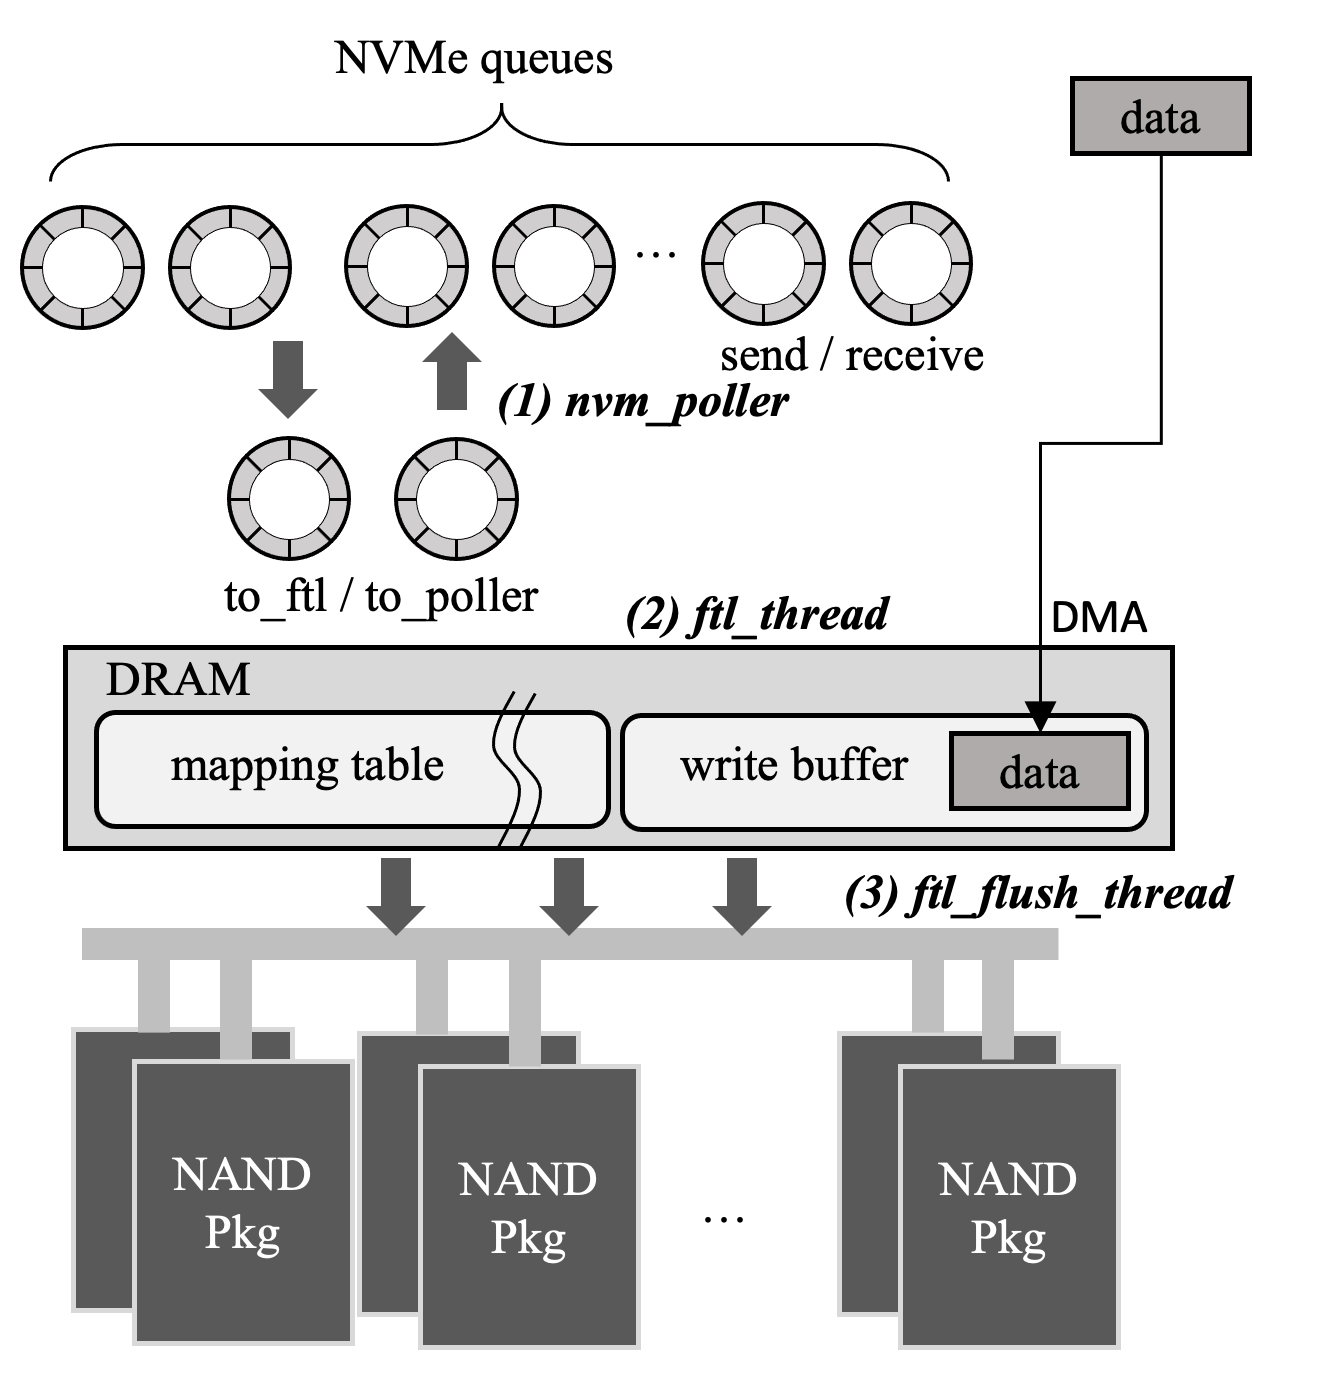
\includegraphics[width=0.3\textwidth]{figure/dawid_ssd_archi_new.eps}
% 	} \\
% 	\subfloat[Data structures for FTL]{ 
%     	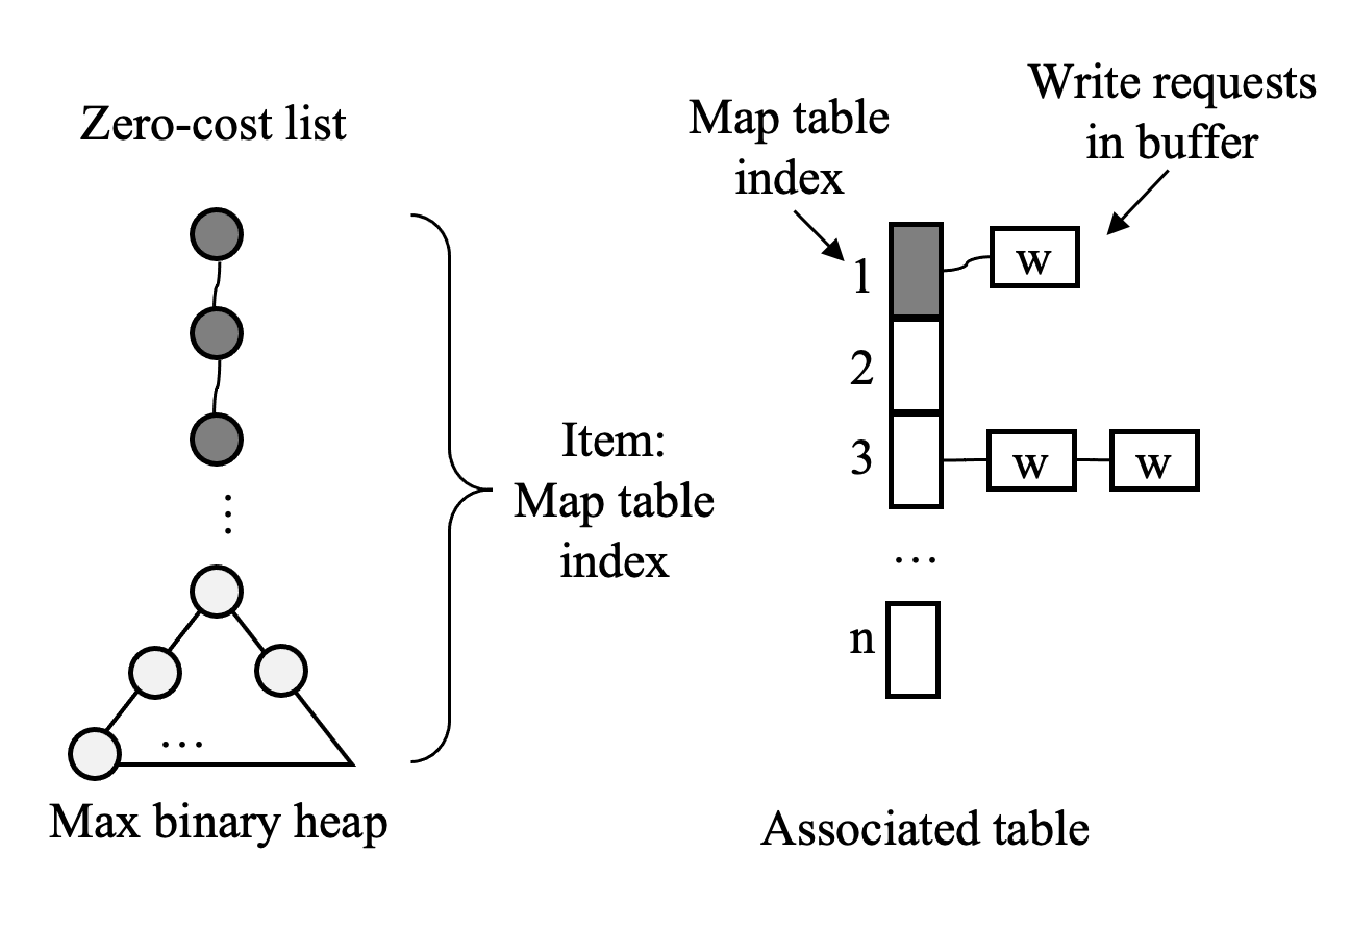
\includegraphics[width=0.3\textwidth]{figure/dawid_ds.eps}
% 	}
    % 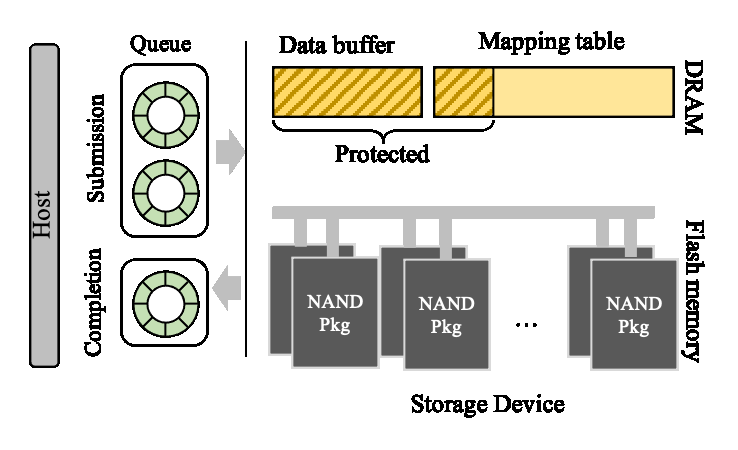
\includegraphics[width=0.4\textwidth]{figure/dawid_ssd_archi.eps}
    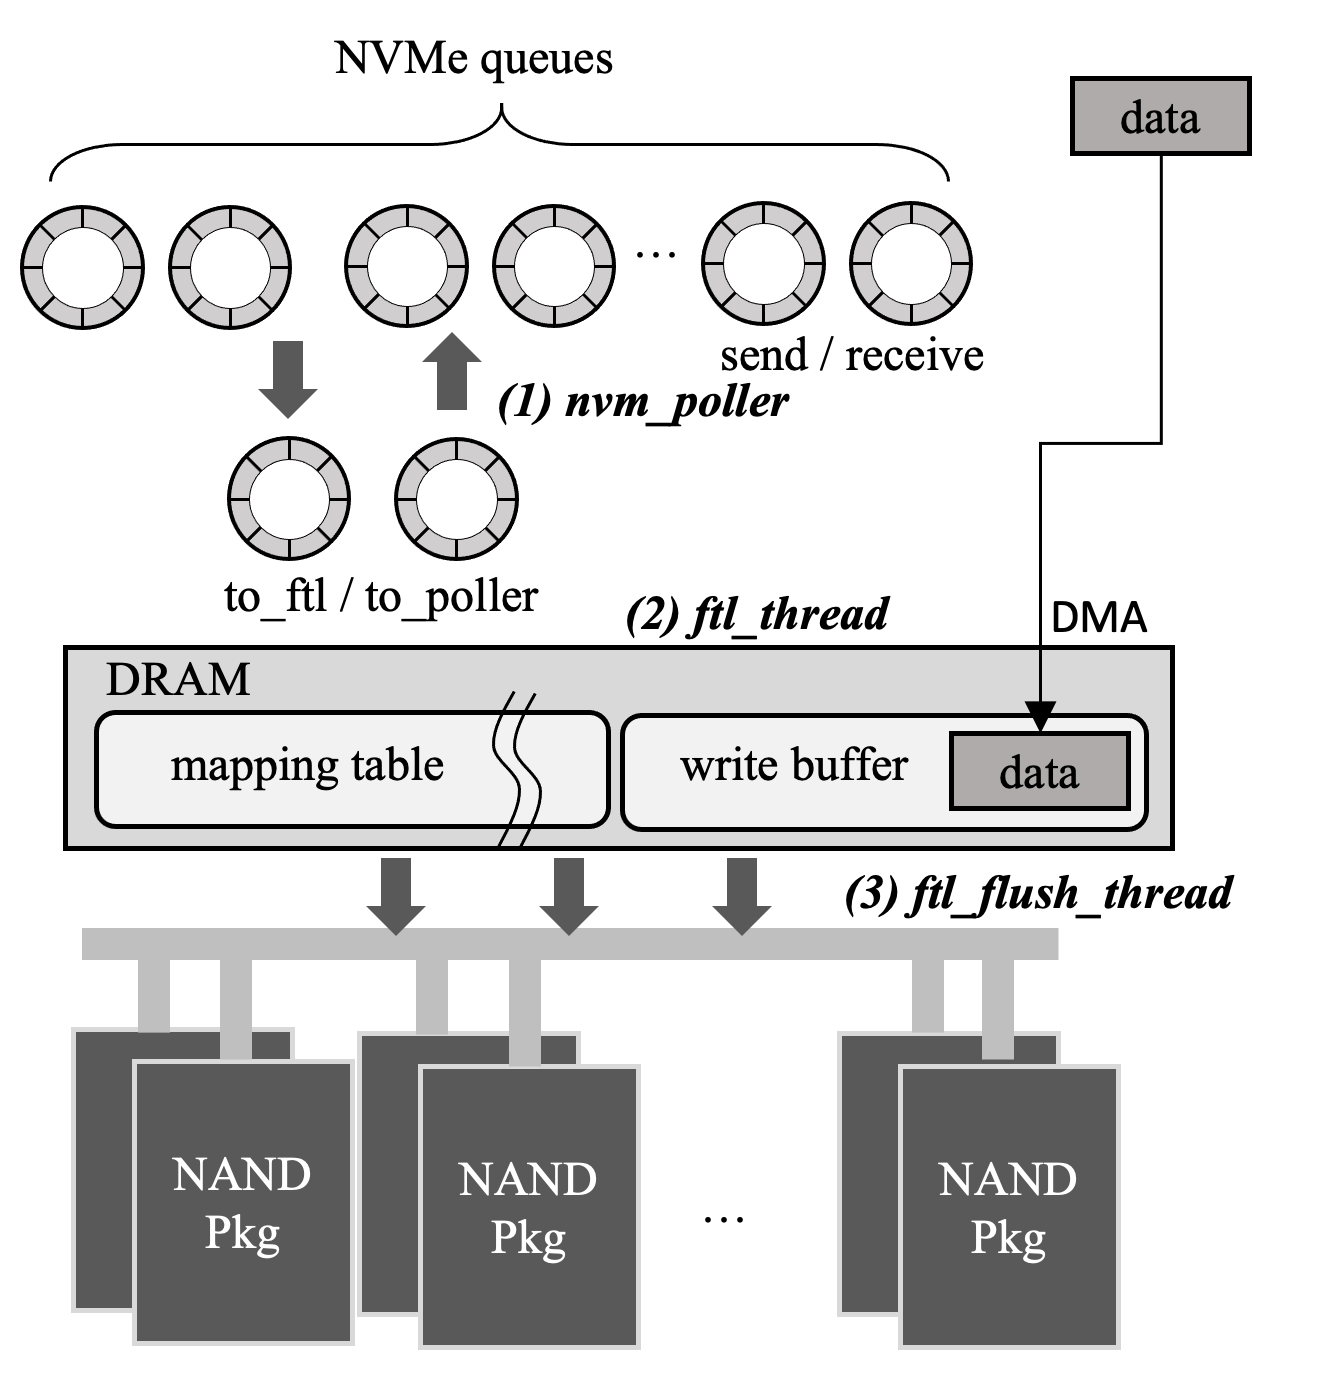
\includegraphics[width=0.3\textwidth]{figure/dawid_ssd_archi_new.eps}
    \caption{\textbf{\ours{} Architecture.}}
    \label{fig_dawid_archi}
    \vspace{-20pt}
\end{figure}

% \section{Implementation}
Fig.~\ref{fig_dawid_archi} shows the overall
architecture of \ours{}. %and its internal data structures. 
\ours{} is implemented by extending \texttt{FEMU}, an open-source SSD development
framework~\cite{li2018case}. 
\ours{} communicates with a host using NVMe storage interfaces and uses a small write buffer, which aggregates and batches user writes into the underlying flash memory.  

% As the original
% version of \texttt{FEMU} directly writes data to flash memories without write
% buffering, we extend it to use a small-sized write buffer, which aggregates and  
% batches user writes into the underlying flash memory.  

\ours{} maintains three different threads that are executing concurrently
within SSDs.  The \texttt{nvm\_poller} takes a charge of transferring requests
between NVMe queues and FTL-internal queues. The FTL-internal queue consists of
a pair of sub-queues, named \texttt{to\_ftl} and
\texttt{to\_poller}. This separation is intended to enable a non-blocking
access to queues by allowing only a single writer for each queue.  Second, the
\texttt{ftl\_thread} essentially handles the ingress requests from the internal
queues. For write, it transfers data from the host memory to the SSD-internal
write buffer with DMA and updates the associated entry in a translation page to
point to the write buffer. Then, it notifies the completion of request to the
\texttt{nvm\_poller} by enqueueing the acknowledgement into the
\texttt{to\_poller} queue.  Because \ours{} protects the entire space of write
buffer with capacitance, data persistency is guaranteed for all acknowledged
writes.  For read, the \texttt{ftl\_thread} retrieves the requested data by
consulting the mapping table and transfers them to the host. 

The \texttt{ftl\_flush\_thread} materializes data from a DRAM-buffer
into a flash memory.  In FIFO-SSD, the user writes are issued
to NAND flash memory in the order they arrive into the buffer. However, \ours{}
flushes buffered writes in the order such that it least increases the dirty memory
footprint of the mapping table.  To realize this design, \ours{} maintains two
data structures, as depicted in Fig.~\ref{fig_dawid_archi}(b). First, \textit{a
zero-cost list} that holds the indexes to translation pages that are already
in a dirty state, and second, \textit{a max binary heap}
maintains the indexes to translation pages sorted by the number of buffered
user-write requests associated with that page.  

%When there is sufficient bandwidth at underlying NAND flash subsystem for writes, 
When half of the write buffer becomes occupied, flushing is invoked. \ours{}
first flushes the user data on those translation pages in the zero-cost list, and then
persists user data as their translation pages are ordered by the max binary
heap. 
%By doing so, each user write minimizes the number of eventual translation page write, and each translation page write maximizes the number of persisted mapping entries. 
These data structures are updated by the \texttt{ftl\_thread} 
when a write request arrives at SSD. 
To exploit the SSD internal parallelism, we send data to flash memory in
batches by the number of NAND flash chips that can be written simultaneously.

Once the write operations of NAND flash memory complete,
\texttt{ftl\_flush\_thread} updates the mapping table entries to point to the
physical address of the data in a flash memory.  At this moment, if the number
of dirty mapping table pages goes beyond the protectable number of pages,
\texttt{ftl\_flush\_thread} persists the mapping table page to flash memory.
This is also conducted in batches by the number of NAND flash chips that can be
written in parallel.
